\documentclass[11pt,a4paper]{article}

\usepackage[margin=20mm]{geometry}
\usepackage{booktabs}
\usepackage{graphicx}
\usepackage{hyperref}
\usepackage{xcolor}
\usepackage{enumitem}
\usepackage{microtype}

\hypersetup{colorlinks=true,linkcolor=black,urlcolor=blue!50!black}
\setlist[itemize]{leftmargin=*,itemsep=2pt,topsep=3pt}
\setlist[enumerate]{leftmargin=*,itemsep=2pt,topsep=3pt}
\setlength{\parskip}{0.35em}
\setlength{\parindent}{0pt}

\title{Moln\'ar Gate~A3 Supervisor Decision Package}
\author{RF--U $h$-convergence at $l_c=0.015$\,mm\\
\small Analysis revision: \texttt{db4c1fa}\\
\small Status: supervisor decision required --- no additional simulations are requested at this stage}
\date{}

\begin{document}
\maketitle

\section*{A. Study completed}

A controlled serial $h$-convergence study was completed for the exact author-supplied supplementary single-notch Moln\'ar model at $l_c=0.015$\,mm.

\begin{center}
\begin{tabular}{@{}ll@{}}
\toprule
Layer & Result \\
\midrule
H0 / H1 / H2-PUB Abaqus solvers & technical pass \\
Consolidated CAE RF--U extraction (\texttt{1376236}) & pass for all three \\
Formal RF--U successive-mesh analysis & complete \\
Matched-state SDV15 / crack-path contours & \textbf{not assessed} (export incomplete) \\
\bottomrule
\end{tabular}
\end{center}

Scientific input revision for the mesh family: \texttt{58d7e3102d76fe0e70e6729457e2c7e90ad131bb}.

This package does \textbf{not} re-open candidate-v2 SDV15 irreversibility as the primary decision. The decisions requested here concern uniform RF--U reference selection for the $l_c=0.015$\,mm supplementary $h$-convergence chain.

\section*{B. Mesh family}

\begin{center}
\begin{tabular}{@{}llrrr@{}}
\toprule
Case & Role & Local $h$ & $N$ & Solver job \\
\midrule
H0 & Exact author supplementary & $\approx 0.00494$\,mm & 3930 & \texttt{1376154} \\
H1 & Intermediate refinement & $0.0025$\,mm & 12064 & \texttt{1376185} \\
H2-PUB & Publication local resolution & $0.001$\,mm & 33852 & \texttt{1376186} \\
\bottomrule
\end{tabular}
\end{center}

H2-PUB targets the publication-reported local crack-path resolution $h=0.001$\,mm. The element count (33852) is generated and is not forced to the approximate paper statement of $\sim 22000$ elements.

\section*{C. Key RF--U results}

\subsection*{Scalar peaks}
\begin{center}
\begin{tabular}{@{}lrr@{}}
\toprule
Case & peak RF2 [kN] & $U_\mathrm{peak}$ [mm] \\
\midrule
H0 & 0.727608 & 0.00610 \\
H1 & 0.699604 & 0.00580 \\
H2-PUB & 0.696336 & 0.00580 \\
\bottomrule
\end{tabular}
\end{center}

\subsection*{Successive-mesh differences (finer mesh = denominator)}
\begin{center}
\begin{tabular}{@{}lrrrrr@{}}
\toprule
Pair & $\Delta F_\mathrm{peak}$ & $\Delta U_\mathrm{peak}$ & full NRMSE & pre-peak NRMSE & post-peak NRMSE \\
\midrule
H0$\to$H1 & $4.003\%$ & $5.172\%$ & $21.306\%$ & $0.387\%$ & $62.904\%$ \\
H1$\to$H2-PUB & $0.469\%$ & $0\%$ & $6.011\%$ & $0.106\%$ & $20.206\%$ \\
\bottomrule
\end{tabular}
\end{center}

Initial stiffness change H1$\to$H2-PUB $\approx 0.06\%$.

\subsection*{Clear statements}
\begin{itemize}
  \item Peak and pre-peak RF--U $h$-convergence between H1 and H2-PUB are \textbf{supported}.
  \item Post-peak mesh dependence \textbf{remains} (full-curve NRMSE $\approx 6\%$ is post-peak-driven).
  \item Do \textbf{not} claim unrestricted full-curve mesh independence.
  \item Crack-path / matched-state SDV15 convergence is \textbf{not assessed}.
\end{itemize}

\begin{quote}
\itshape
The force--displacement response is effectively mesh-independent between H1 and H2-PUB for the elastic, pre-peak and peak-load regimes. A noticeable post-peak mesh dependence remains and must be retained as a limitation.
\end{quote}

\begin{center}
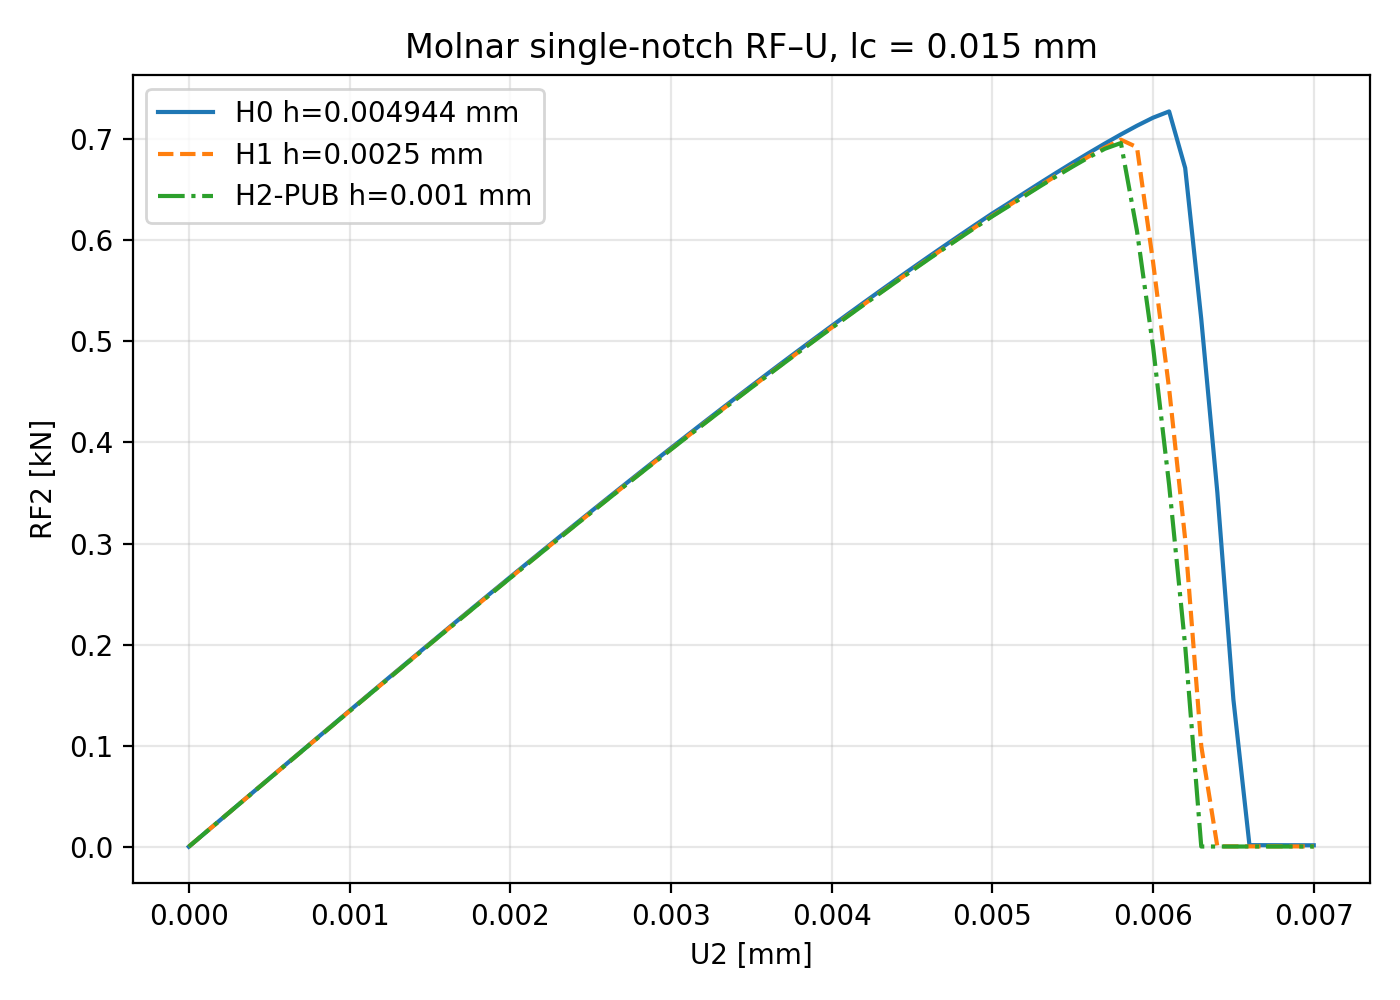
\includegraphics[width=0.95\textwidth]{../../results/figures/molnar_lc015_h_convergence/01_rf_u_h0_h1_h2.png}
\end{center}

\section*{D. Publication comparison}

Reference used: an approximate digitization of the Moln\'ar Fig.~7 curve for $l_c=0.015$\,mm.
It is not exact author numerical data. The $l_c=0.0075$\,mm curve was not used.

\begin{center}
\begin{tabular}{@{}lrr@{}}
\toprule
Case & Full-overlap NRMSE vs Fig.~7 ($l_c=0.015$) & $\Delta F_\mathrm{peak}$ vs ref \\
\midrule
H0 & $\sim 25.3\%$ & $\sim +5.4\%$ \\
H1 & $\sim 18.4\%$ & $\sim +1.3\%$ \\
H2-PUB & $\sim 15.6\%$ & $\sim +0.8\%$ \\
\bottomrule
\end{tabular}
\end{center}

Publication agreement is \textbf{provisional} and secondary to successive-mesh evidence.

\section*{E. Computational cost (serial)}

\begin{center}
\begin{tabular}{@{}lrrr@{}}
\toprule
Case & $N$ & Walltime & Peak memory (approx.) \\
\midrule
H0 & 3930 & 00:16:29 & $\sim 0.68$\,GB \\
H1 & 12064 & 00:46:26 & $\sim 0.91$\,GB \\
H2-PUB & 33852 & 02:12:38 & $\sim 1.76$\,GB \\
\bottomrule
\end{tabular}
\end{center}

H1 uses about \textbf{35\% of H2-PUB walltime} while nearly matching H2 peak and pre-peak RF--U response.

\section*{F. Remaining limitations}
\begin{enumerate}
  \item Post-peak RF--U residual between H1 and H2-PUB ($\sim 20\%$ post-peak NRMSE).
  \item Matched-state SDV15 / crack-path contour exports incomplete for all three meshes.
  \item Fig.~7 comparison is approximate digitization only.
  \item Supervisor-approved numerical tolerances are not yet fixed.
  \item Candidate-v2 SDV15 accepted-increment irreversibility remains a separate documented issue for the paper-matched route (not the primary request of this package).
\end{enumerate}

\section*{G. Decisions requested (exactly two)}

\subsection*{Decision 1 --- Uniform RF--U reference}
Please choose one:
\begin{itemize}
  \item[\textbf{A}] Accept \textbf{H2-PUB ($h=0.001$\,mm)} as the uniform RF--U reference.
  \item[\textbf{B}] Accept \textbf{H2-PUB provisionally}, subject to contour evidence.
  \item[\textbf{C}] Do \textbf{not} accept; specify additional required evidence.
\end{itemize}
Project recommendation: option A or B, with H2-PUB as the conservative RF--U reference; H1 for intermediate development; H0 not a final reference.

\subsection*{Decision 2 --- Contour requirement}
Please choose one:
\begin{itemize}
  \item[\textbf{A}] Matched-state SDV15 / crack-path contours are \textbf{mandatory} before Gate~A3 closes.
  \item[\textbf{B}] Contours may be \textbf{deferred}; RF--U evidence is sufficient to proceed \textbf{conditionally} to MISESERI preparation.
  \item[\textbf{C}] Contours required only for \textbf{H1 and H2-PUB}.
  \item[\textbf{D}] Other requirement specified by the supervisor.
\end{itemize}
No supervisor answer is inferred. No route is executed by this package alone.

\section*{H. Consequences of each route}

\subsection*{Route A --- H2-PUB accepted and contours waived/deferred (Decision 1 A/B + Decision 2 B)}
\begin{itemize}
  \item Gate~A3 may be closed or conditionally waived (supervisor wording required).
  \item Freeze H2-PUB as the RF--U uniform reference.
  \item Allow preparation only of Stage~C / MISESERI workflow documentation.
  \item No solver/MISESERI execution until a separate submission plan is approved.
\end{itemize}

\subsection*{Route B --- Contours mandatory (Decision 2 A or C)}
\begin{itemize}
  \item Gate~A3 remains open.
  \item Prepare a contour-only postprocessing repair using existing H0/H1/H2 ODBs.
  \item No solver rerun.
  \item Request separate authorization for one CAE-only contour extraction job.
\end{itemize}

\subsection*{Route C --- Additional numerical evidence (Decision 1 C or Decision 2 D)}
\begin{itemize}
  \item Document the exact requested metric.
  \item Prepare a new scoped plan.
  \item Do not submit anything automatically.
\end{itemize}

\section*{Current project boundary}
\begin{itemize}
  \item H2-PUB RF--U reference: recommended (awaiting Decision~1)
  \item H1 intermediate mesh: recommended
  \item Post-peak convergence: limited / not fully demonstrated
  \item Crack-path convergence: not assessed
  \item Gate~A3: supervisor decision pending (overall open; historical label \texttt{reference\_data\_insufficient}; RF--U component \texttt{rf\_u\_reference\_supported\_contour\_evidence\_pending})
  \item New HPC authorization: none
  \item MISESERI / remeshing / state transfer: blocked
\end{itemize}

\end{document}
